%%% fs-run-time-impl Implementation
\label{fs-impl}

\subsection{Ordering model}
The meta-information of data item is a tuple of a {\it global time}, a {\it trace}, {\it child ids} and a tombstone flag.

\[Meta := (GlobalTime, ChildIds[], Trace, IsTombstone)\]

Global time is assigned to data item once the item enters the system. It is a pair of milliseconds since the epoch start and the identifier of the front. The identifier is used to assign different global times to different items, even in case of wall-clock collisions. 

\[GlobalTime := (FrontTs, FrontId)\]

Global times are compared by front timestamp if they coincide - by front id. It is important to notice that we do not rely on any clock synchronization between nodes, but we require strict monotonicity within the single front. The only implication of the clock skew is the system degradation regarding latency: 1ms of the nodes clock difference appends 1 ms to minimal latency.

Each map operation can produce multiple items from one. To differentiate them the ordinal number, {\it child id}, is stored in the meta information. The {\it ChildIds } is an array of child ids, that corresponds to the all visited map operations.

The global time and child ids are enough to uniquely identify data item within stream if all processing is done without replays. If there are any replays happened during processing, multiple items with the same global time and child ids exist in the stream. Multiple tombstones with the same global time and child ids can exist as well. They can take different paths in computational flow and travel within them with different speeds. 

Despite this fact, an invalid element and the corresponding tombstone go along the same path, because they have the same payload and the balancing functions are deterministic. Moreover, the tombstone visits operations strictly after corresponding item, as links between operation are expected to be FIFO. 

To match tombstone with proper item, there is {\it Trace} value stored in the meta-information. Trace encodes the path that item have traversed. The unique random 64-bit identifier is assigned to each physical operation. The trace is a xor of all operations' ids visited by item so far.

%TODO: uncomment
%\[Trace := \bigoplus_{op \in \text{visited}} Id(op)\]

Metas are compared lexicographically: firstly global times are compared, then child ids, then traces. Notably, this order is in line with the \FlameStream's ordering model.

Figure~\ref{logical-graph-ops-figure} shows the topology of each operation and how it affects the meta. Grouping and merge operations update trace of the data item by xoring initial trace with its physical id. Map and broadcast apply the same update, but also append child id for each output item.

\begin{figure}[htbp]
  \centering
  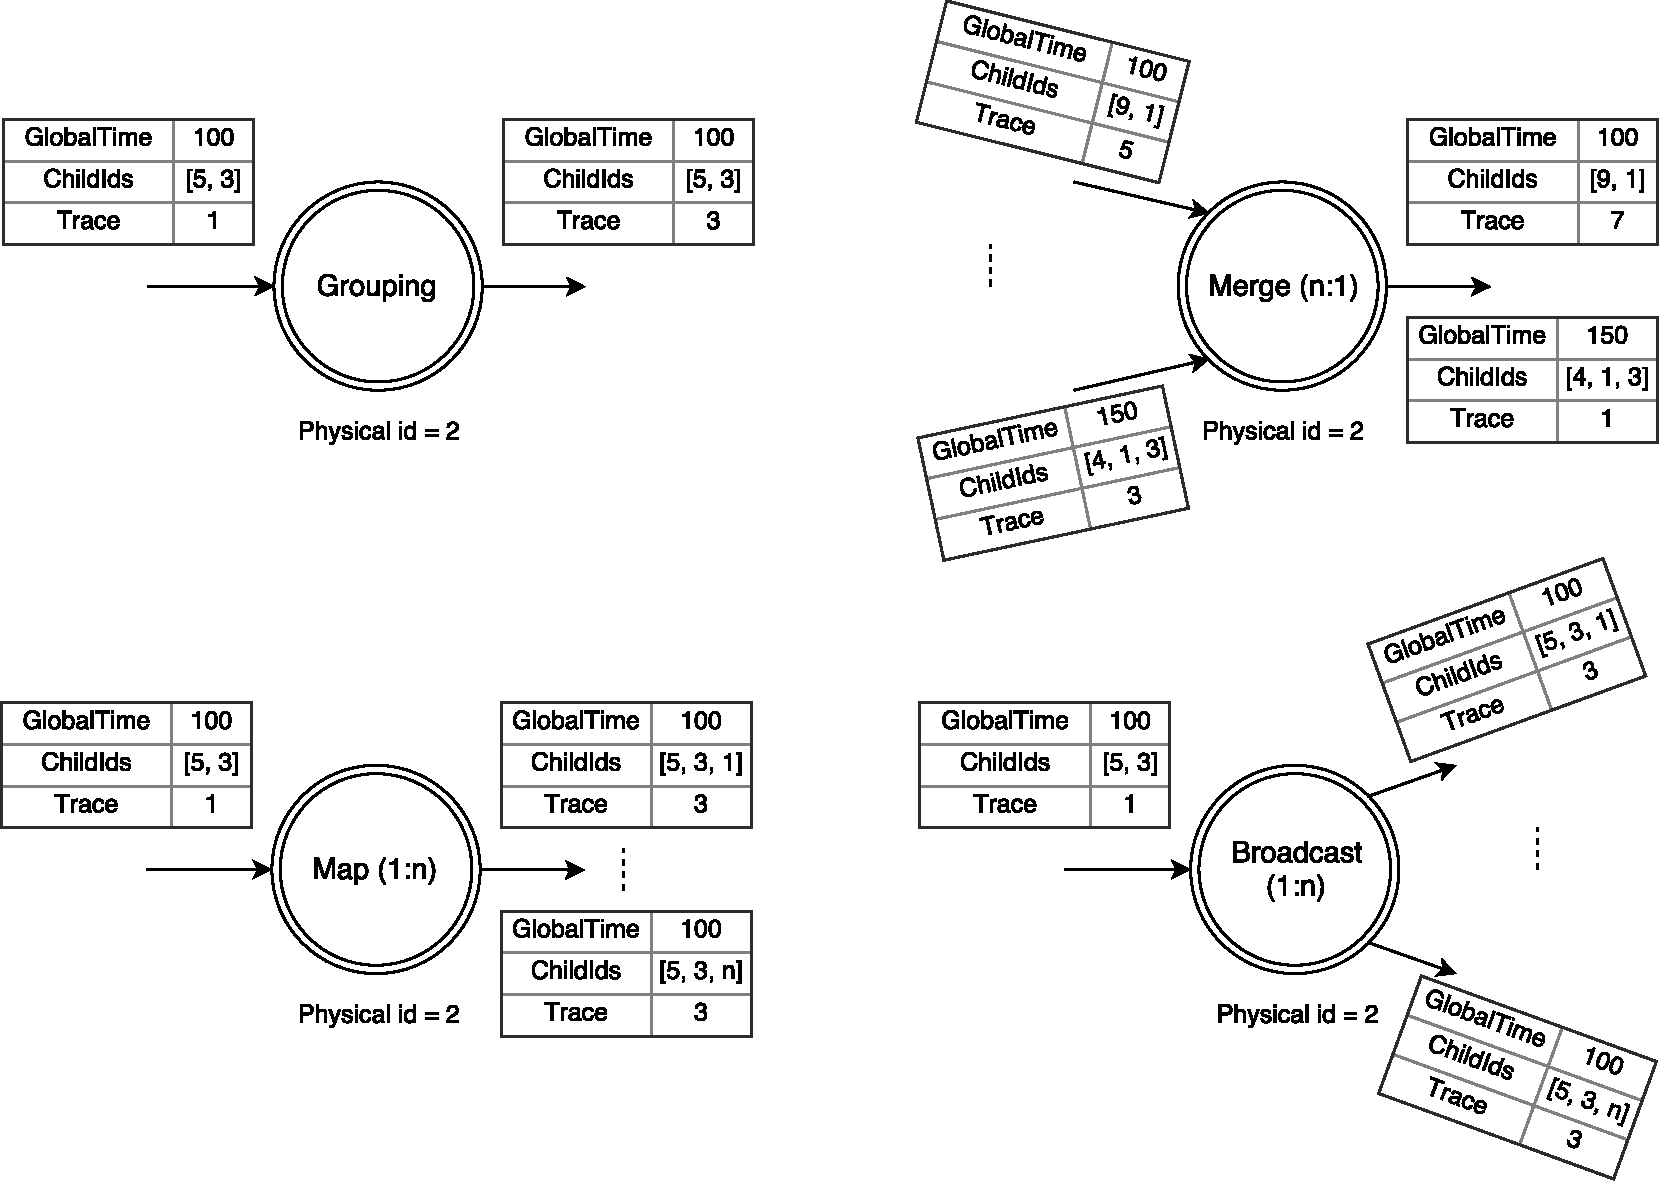
\includegraphics[scale=0.5]{pics/operations}
  \caption{The topology of each operation and how it affects the meta}
  \label {logical-graph-ops-figure}
\end{figure}

The structure of meta provides for tracking different relations between data items:

\begin{itemize}
  \item Items with same global time and common prefixes are produced from the same item
  \item Item with lower meta is generated earlier, at front or in the stream
  \item If there are two items with the same global time and child ids, only one of them is the valid one
\end{itemize}

\label{mininal-time}

\subsection{Minimal time within stream}

To release the item from the barrier we need to ensure that there are no in-flight tombstones. 

\newtheorem{minimal-time-claim}{Lemma}

\begin{minimal-time-claim}
  If data item {\it D} has global time {\it GT} greater than the global time of each in-flight element, then all tombstones for that item had already arrived at the barrier.
\end{minimal-time-claim}

\begin{proof}
  Let $D_{tomb}$ be an in-flight tombstone for {\it D}. According to the definition of the tombstone item, $D_{tomb}$ and {\it D} has the same global time {\it GT}. We assumed that there are no in-flight element with the global time equal to {\it GT}. Contradiction.
  
  New tombstones for {\it D} cannot be generated because items with global time greater than {\it GT} cannot trigger replay that affects {\it D}.

  This implies that if the stream does not contain items with the global time less than or equal to {\it GT}, then all tombstones for {\it D} had already arrived at the barrier. 
\end{proof}

Therefore, to output an item from the barrier, we should ensure that there are no items in the stream with the global time less than or equal to the global time of this item.

To track the global time of in-flight items we adopt an idea of {\it acker task} inspired by Apache Storm~\cite{apache:storm}. Acker tracks data items using a checksum hash. When the item is sent or received by an operation, its global time and checksum are sent to the acker. This message is called {\it ack}. Acker groups acks by a global time into the structure called {\it ack table}. Once acker receives an ack message with global time {\it GT} and {\it XOR} it updates {\it GT} entry in the table by xoring {\it XOR} with the current value. When an item is sent and later received by the next operation, xoring corresponding {\it XOR}s would yield zero.

Acks are overlapped to nullify table's entry only when an item arrives at the barrier. That is, ack for receive is sent only after both processing and the ack sending for the transformed item, as illustrated in Figure~\ref{acker}. Different shapes of items mean different payloads. The ack for the sending of the triangular element is sent before the rectangular one. We expect the channel between the acker and each operation to be FIFO, so ack for the triangular item would be xored before the rectangular. So the two equal values are separated by distinct one. 

This technique guarantees that the {\it XOR} for some global time is equal to zero only if there are no in-flight elements with such global time.

\begin{figure}[htbp]
  \centering
  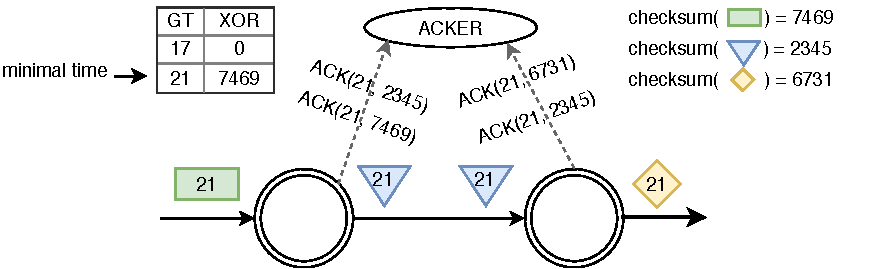
\includegraphics[scale=0.6]{pics/acker}
  \caption{The example of tracking minimal time using acker}
  \label {acker}
\end{figure}

The minimal time within a stream is the minimal global time with non-zero {\it XOR}. On minimal time changes, acker broadcasts new minimal time to the barrier and operations. Therefore, the barrier can release elements with global time {\it GT} once it received notification from acker that the minimal time within the stream is greater than {\it GT}.

To ensure that no fronts can generate item with the specific timestamp, each front periodically sends to acker special message called {\it report}, which promises that front will not generate items with a timestamp lower than the reported. The value in the ack table can become zero only after the corresponding report arrives.

The proposed mechanism could be isolated by hash range. This change allows us releasing from barriers on different workers independently. This feature is also known as early key availability.

\subsection{Distributed runtime}

\FlameStream\ is implemented in Java, using Akka framework for messaging and Apache Zookeeper for cluster state management. The usage of Zookeeper mitigates the need for the dedicated master node.

From a user perspective, the system provides an API to define processing in terms of {\it ticks}. Tick is represented by a time interval and the graph that handles data items, which relate to this interval, according to the global time. To deploy a tick, the client writes it directly to Zookeeper, whereas Zookeeper notifies workers when the new tick appears. As soon as tick ends, the system starts to execute the next one if any was submitted to Zookeeper. Otherwise, processing is completely stopped.

The underlying purpose of ticks is to provide an ability to rebuild and redeploy graph periodically. We keep in mind that the possible client of FlameStream is a system that automatically builds a graph based on declarative language. However, such system cannot build it once and use without modifications, because the performance of graph execution can be influenced by the current load, the performance of operations, metrics, etc. Hence, frequent graph redeployment is crucial for our system. 

\subsection{Fault tolerance}
Currently, fault tolerance mechanisms are not among the goals of our prototype. However, it is worth to share how they can be implemented in our system.

Typically, distributed systems take into consideration the following types of failures:
\begin{itemize}
    \item Packet loss
    \item Node failure
    \item Network partitioning
\end{itemize}

Acker can determine the packet loss issue if it happens. Therefore, the part of the stream can be replayed by the fronts subsystem if it supports some reliable buffer.

Node failure also can be readily determined by the acker. The only difficulty is the loss of the grouping state. Hence, there is a need for grouping state replication.

Support of network partitioning tolerance is not planned because it leads to an unavoidable loss of data. We believe that in this case, stream processing does not make sense.
